\documentclass[aspectratio=169,10pt]{beamer}

\usepackage[utf8]{inputenc}
\usepackage[T1]{fontenc}
\usepackage[french]{babel}
\usepackage{graphicx}
\usepackage{booktabs}
\usepackage{array}

\usetheme{Madrid}
\usecolortheme{default}

\definecolor{primary}{HTML}{1E3A8A}
\definecolor{accent}{HTML}{059669}
\definecolor{softgray}{HTML}{F3F4F6}
\definecolor{darkgray}{HTML}{374151}

\setbeamercolor{structure}{fg=primary}
\setbeamercolor{frametitle}{bg=primary,fg=white}
\setbeamercolor{title}{fg=primary}
\setbeamercolor{block title}{bg=primary,fg=white}
\setbeamercolor{block body}{bg=softgray,fg=black}
\setbeamertemplate{navigation symbols}{}
\setbeamertemplate{itemize item}{\color{accent}$\blacktriangleright$}
\setbeamertemplate{itemize subitem}{\color{primary}$\bullet$}

\graphicspath{{./}}

\title[Agent MCP CRM Bitext]{Agent MCP CRM Bitext}
\subtitle{Support client intelligent basé sur la classification d'intentions et les tools MCP}
\author[BENABOU, COMPAORE, DIALLO]{
BENABOU Hafsa \and COMPAORE Moustapha \and DIALLO Mamadou Tahirou
}
\institute[INPT]{Institut National des Postes et Télécommunications\\Filière Sciences de Données -- 2ème année Ingénieur}
Mini-projet INE
\topic{Mise en place d'une aoi Agent MCP           
Support client intelligent basé sur la classi?cation d'intentions, les tools
MCP et Ollama}
\date{Juin 2026}

\begin{document}

\begin{frame}
    \titlepage
    \vspace{-0.6cm}
    \begin{center}
        
\includegraphics[height=0.9cm]{Logo_ANRT_NV.jpg}
        \hspace{1.8cm}
        
\includegraphics[height=0.9cm]{Logo_inpt.PNG}
    \end{center}
\end{frame}

\begin{frame}{Plan de la présentation}
    \begin{columns}[T]
        \begin{column}{0.48\textwidth}
            \begin{enumerate}
                \item Contexte et objectif
                \item Données utilisées
                \item Architecture générale
                \item Classification d'intentions
            \end{enumerate}
        \end{column}
        \begin{column}{0.48\textwidth}
            \begin{enumerate}
                \setcounter{enumi}{4}
                \item Mapping MCP et agent CRM
                \item API, interface et déploiement
                \item Évaluation
                \item Bilan et perspectives
            \end{enumerate}
        \end{column}
    \end{columns}
\end{frame}

\begin{frame}{Problématique}
    \begin{block}{Question de départ}
        Comment automatiser une partie du support client tout en gardant une réponse structurée, traçable et exploitable par un système CRM ?
    \end{block}

    \vspace{0.2cm}
    \begin{columns}[T]
        \begin{column}{0.48\textwidth}
            \textbf{Besoins côté client}
            \begin{itemize}
                \item annuler ou suivre une commande ;
                \item demander une facture ou un remboursement ;
                \item modifier une adresse ;
                \item contacter un agent humain.
            \end{itemize}
        \end{column}
        \begin{column}{0.48\textwidth}
            \textbf{Besoins côté système}
            \begin{itemize}
                \item comprendre l'intention ;
                \item appeler le bon outil métier ;
                \item produire une réponse claire ;
                \item fonctionner sur une machine CPU.
            \end{itemize}
        \end{column}
    \end{columns}
\end{frame}

\begin{frame}{Objectif du projet}
    \begin{center}
        \large
        \textbf{Construire un agent CRM modulaire capable de traiter une demande client de bout en bout.}
    \end{center}

    \vspace{0.25cm}
    \begin{block}{Pipeline cible}
        Message utilisateur
        $\rightarrow$ classification de l'intention
        $\rightarrow$ sélection du tool MCP
        $\rightarrow$ exécution CRM
        $\rightarrow$ réponse finale
    \end{block}

    \vspace{0.2cm}
    \begin{itemize}
        \item Une solution reproductible : scripts, API, interface et documentation.
        \item Une solution pragmatique : modèle léger TF-IDF + LogisticRegression sur CPU.
        \item Une solution extensible : variante Transformer et reformulation optionnelle avec Ollama.
    \end{itemize}
\end{frame}

\begin{frame}{Choix du dataset}
    \begin{table}
        \small
        \begin{tabular}{>{\bfseries}p{0.28\textwidth}p{0.24\textwidth}p{0.38\textwidth}}
            \toprule
            Dataset & Utilité & Décision \\
            \midrule
            Telco Customer Churn & Prédiction du churn client & Intéressant pour un futur tool de scoring, mais pas centré sur les messages. \\
            92k Call Center Scripts & Corpus conversationnel riche & Utile pour RAG ou mémoire, mais moins direct pour la classification d'intentions. \\
            Bitext Customer Support Chatbot & 26 900 paires instruction/réponse, 27 intentions & Retenu comme dataset principal du projet. \\
            \bottomrule
        \end{tabular}
    \end{table}

    \vspace{0.1cm}
    \begin{block}{Pourquoi Bitext ?}
        Il correspond directement au besoin : entraîner un classificateur d'intentions et router chaque intention vers une action CRM.
    \end{block}
\end{frame}

\begin{frame}{Analyse exploratoire}
    \begin{columns}[T]
        \begin{column}{0.55\textwidth}
            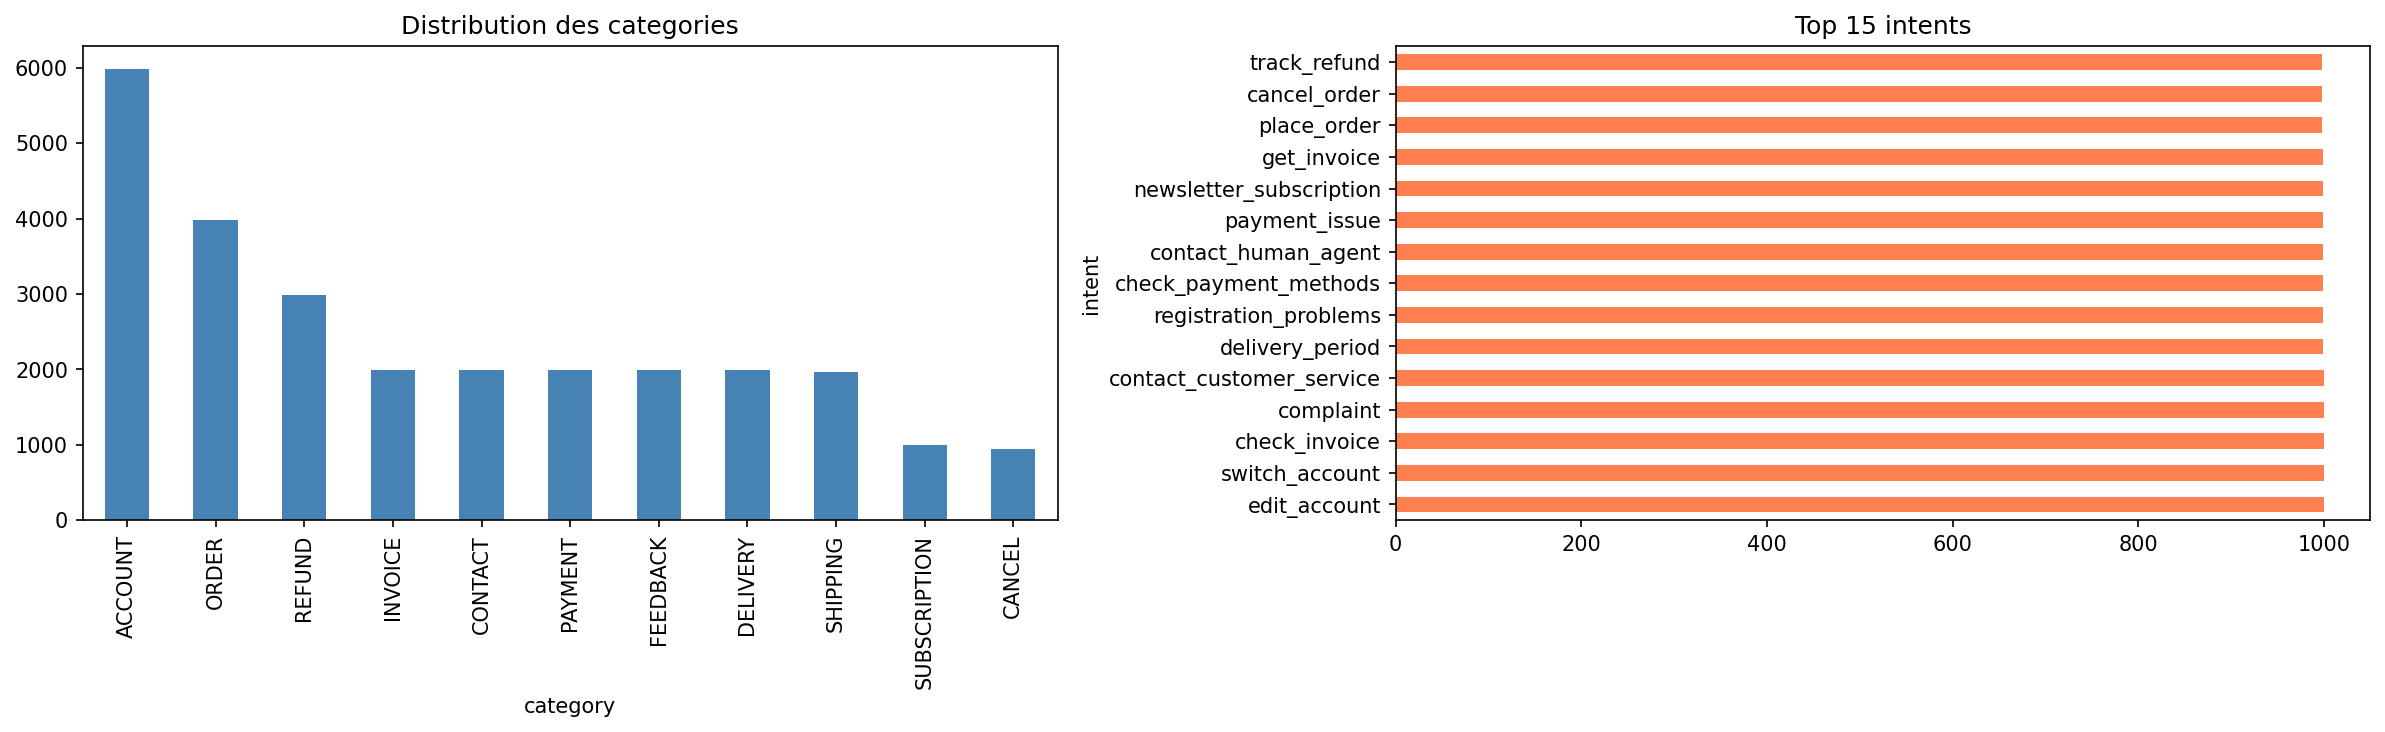
\includegraphics[width=\textwidth]{distribution_dataset.png}
        \end{column}
        \begin{column}{0.43\textwidth}
            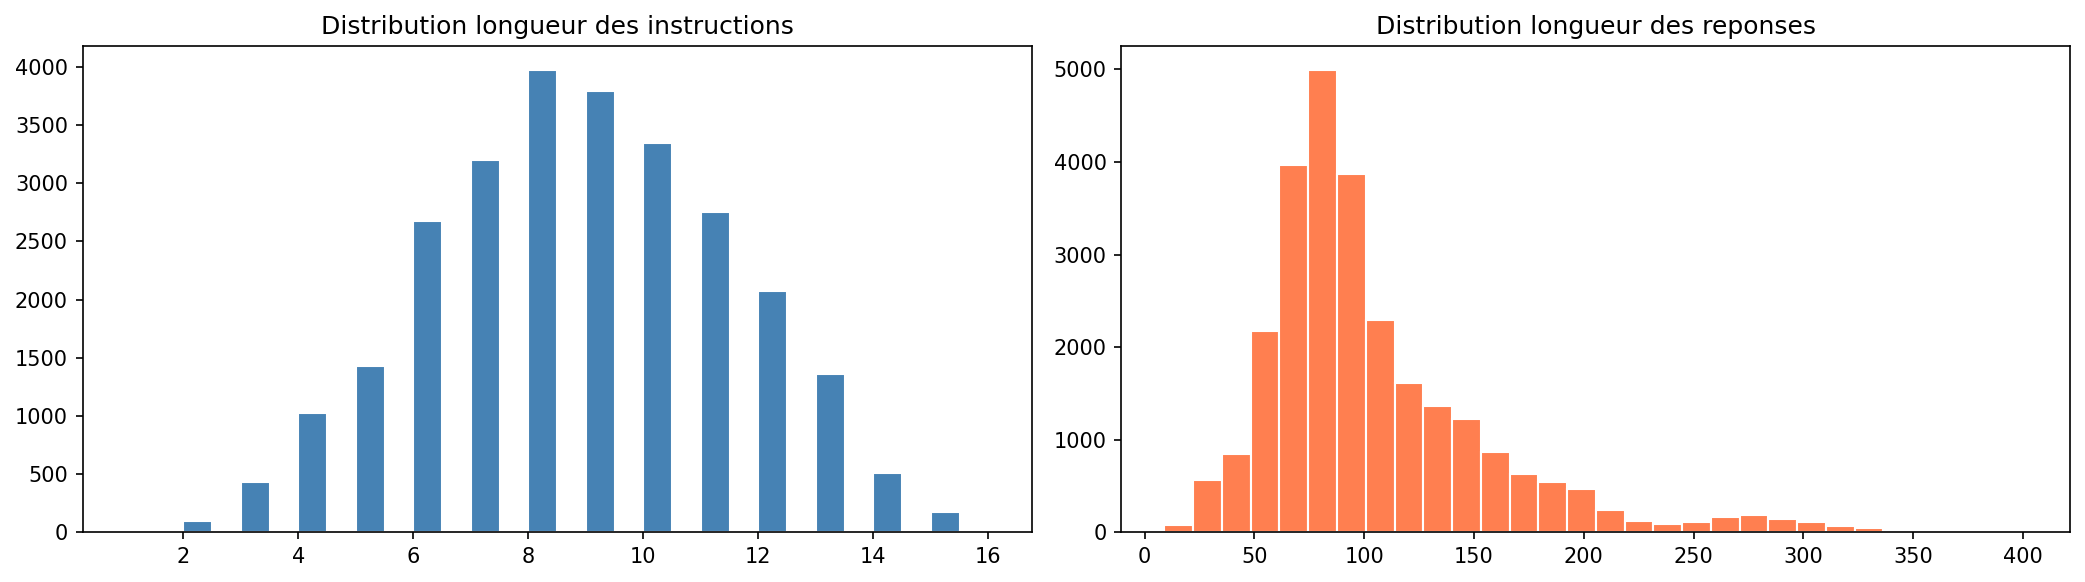
\includegraphics[width=\textwidth]{longueurs_texte.png}
            \vspace{0.2cm}

            \begin{itemize}
                \item analyse des intentions et catégories ;
                \item nettoyage des templates ;
                \item splits train / validation / test ;
                \item génération des fichiers CSV et JSONL.
            \end{itemize}
        \end{column}
    \end{columns}
\end{frame}

\begin{frame}{Architecture générale}
    \begin{columns}[T]
        \begin{column}{0.48\textwidth}
            \begin{block}{Composants}
                \begin{itemize}
                    \item \texttt{data/} : dataset et artefacts ;
                    \item \texttt{src/} : logique métier ;
                    \item \texttt{scripts/} : préparation, entraînement, évaluation ;
                    \item \texttt{api.py} : service FastAPI ;
                    \item \texttt{streamlit\_app.py} : interface de démonstration.
                \end{itemize}
            \end{block}
        \end{column}
        \begin{column}{0.48\textwidth}
            \begin{block}{Flux}
                \begin{enumerate}
                    \item Préparer le dataset Bitext.
                    \item Entraîner le classificateur.
                    \item Mapper l'intention vers un tool MCP.
                    \item Orchestrer la réponse via l'agent.
                    \item Exposer le tout via API et Streamlit.
                \end{enumerate}
            \end{block}
        \end{column}
    \end{columns}
\end{frame}

\begin{frame}{Classification d'intentions}
    \begin{columns}[T]
        \begin{column}{0.52\textwidth}
            \textbf{Modèle principal}
            \begin{itemize}
                \item TF-IDF avec unigrammes et bigrammes ;
                \item maximum de 10 000 features ;
                \item LogisticRegression ;
                \item sauvegarde dans \texttt{data/intent\_classifier.pkl}.
            \end{itemize}

            \vspace{0.2cm}
            \textbf{Pourquoi ce choix ?}
            \begin{itemize}
                \item rapide à entraîner ;
                \item robuste comme baseline ;
                \item adapté aux contraintes CPU.
            \end{itemize}
        \end{column}
        \begin{column}{0.44\textwidth}
            \begin{block}{Variante optionnelle}
                \begin{itemize}
                    \item mini-BERT : \texttt{google/bert\_uncased\_L-2\_H-128\_A-2} ;
                    \item DistilBERT possible ;
                    \item plus coûteux que TF-IDF sur CPU.
                \end{itemize}
            \end{block}
        \end{column}
    \end{columns}
\end{frame}

\begin{frame}{Mapping MCP : de l'intention vers l'action}
    \begin{table}
        \small
        \begin{tabular}{>{\bfseries}p{0.28\textwidth}p{0.32\textwidth}p{0.28\textwidth}}
            \toprule
            Intention & Tool MCP appelé & Paramètres \\
            \midrule
            \texttt{cancel\_order} & \texttt{cancel\_order} & \texttt{order\_id} \\
            \texttt{track\_order} & \texttt{get\_order\_status} & \texttt{order\_id} \\
            \texttt{change\_shipping\_address} & \texttt{update\_shipping\_address} & \texttt{order\_id}, \texttt{new\_address} \\
            \texttt{get\_refund} & \texttt{process\_refund} & \texttt{order\_id}, \texttt{reason} \\
            \texttt{contact\_human\_agent} & \texttt{escalate\_to\_human} & \texttt{reason} \\
            \bottomrule
        \end{tabular}
    \end{table}

    \begin{block}{Idée clé}
        Le modèle ne décide pas directement d'une réponse finale : il choisit une intention, puis l'agent appelle un tool métier explicite.
    \end{block}
\end{frame}

\begin{frame}{Orchestration de l'agent CRM}
    \begin{columns}[T]
        \begin{column}{0.5\textwidth}
            \begin{enumerate}
                \item Recevoir le message utilisateur.
                \item Prédire l'intention et la confiance.
                \item Appliquer un fallback si la confiance est faible.
                \item Extraire les paramètres simples.
                \item Exécuter le tool MCP.
                \item Générer ou retourner la réponse.
            \end{enumerate}
        \end{column}
        \begin{column}{0.46\textwidth}
            \begin{block}{Exemple}
                \texttt{I need to cancel my order \#12345}

                \vspace{0.2cm}
                \textbf{Intent :} \texttt{cancel\_order}

                \textbf{Tool :} \texttt{cancel\_order(order\_id)}

                \textbf{Réponse :} confirmation structurée ou reformulation Ollama.
            \end{block}
        \end{column}
    \end{columns}
\end{frame}

\begin{frame}{API FastAPI et interface Streamlit}
    \begin{columns}[T]
        \begin{column}{0.48\textwidth}
            \textbf{API FastAPI}
            \begin{itemize}
                \item \texttt{GET /health}
                \item \texttt{POST /chat}
                \item \texttt{DELETE /session/\{session\_id\}}
                \item \texttt{GET /intents}
            \end{itemize}

            \vspace{0.2cm}
            Les sessions sont gardées en mémoire pour conserver un historique conversationnel.
        \end{column}
        \begin{column}{0.48\textwidth}
            \textbf{Interface Streamlit}
            \begin{itemize}
                \item test d'un message client ;
                \item affichage de l'intention et de la confiance ;
                \item visualisation du tool MCP appelé ;
                \item dashboard de session ;
                \item export de l'historique.
            \end{itemize}
        \end{column}
    \end{columns}
\end{frame}

\begin{frame}{Évaluation}
    \begin{columns}[T]
        \begin{column}{0.54\textwidth}
            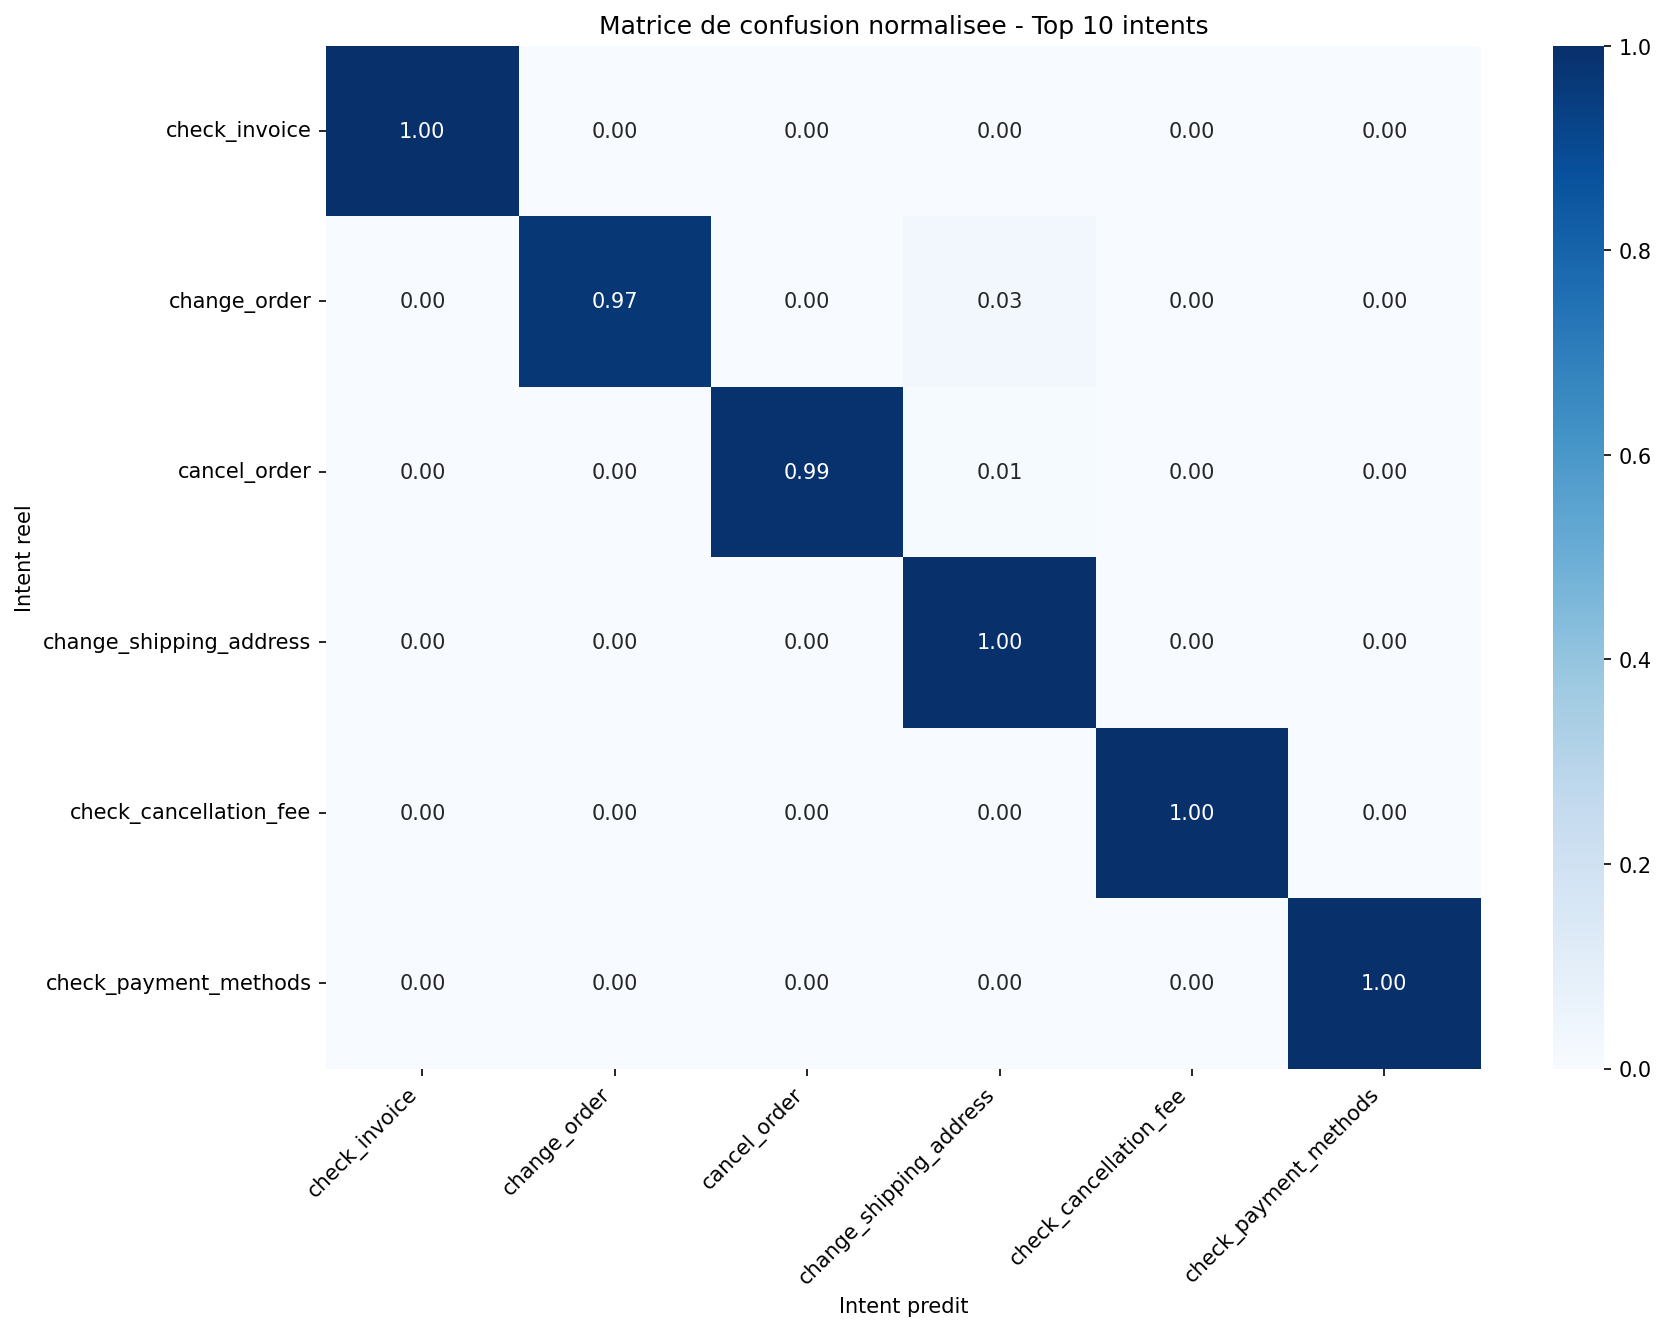
\includegraphics[width=\textwidth]{confusion_matrix.png}
        \end{column}
        \begin{column}{0.42\textwidth}
            \begin{block}{Mesures prévues}
                \begin{itemize}
                    \item accuracy globale ;
                    \item confiance moyenne ;
                    \item ratio de prédictions avec confiance $>80\%$ ;
                    \item rapport de classification ;
                    \item matrice de confusion.
                \end{itemize}
            \end{block}

            \vspace{0.2cm}
            Les tests fonctionnels couvrent le classificateur, le mapping MCP, l'API, Streamlit et les cas limites.
        \end{column}
    \end{columns}
\end{frame}

\begin{frame}{Démonstration proposée}
    \begin{block}{Scénario court à présenter}
        \begin{enumerate}
            \item Lancer l'API FastAPI.
            \item Ouvrir l'interface Streamlit.
            \item Envoyer : \texttt{I want to cancel my order number 12345}.
            \item Montrer l'intention \texttt{cancel\_order}, le score de confiance et le tool appelé.
            \item Tester un message ambigu pour montrer l'escalade vers un humain.
        \end{enumerate}
    \end{block}

    \vspace{0.2cm}
    \begin{columns}
        \begin{column}{0.48\textwidth}
            \textbf{Commande API :}\\
            \texttt{uvicorn api:app --reload --port 8000}
        \end{column}
        \begin{column}{0.48\textwidth}
            \textbf{Commande interface :}\\
            \texttt{streamlit run streamlit\_app.py}
        \end{column}
    \end{columns}
\end{frame}

\begin{frame}{Bilan du projet}
    \begin{columns}[T]
        \begin{column}{0.5\textwidth}
            \textbf{Réalisé}
            \begin{itemize}
                \item projet Python modulaire ;
                \item workflow dataset reproductible ;
                \item classificateur TF-IDF entraînable ;
                \item mapping MCP complet ;
                \item agent CRM fonctionnel ;
                \item API FastAPI et interface Streamlit ;
                \item mode Ollama et mode sans Ollama.
            \end{itemize}
        \end{column}
        \begin{column}{0.46\textwidth}
            \textbf{Limites}
            \begin{itemize}
                \item tools CRM simulés ;
                \item extraction de paramètres simple ;
                \item sessions en mémoire ;
                \item intentions multiples non gérées ;
                \item Transformer encore optionnel.
            \end{itemize}
        \end{column}
    \end{columns}
\end{frame}

\begin{frame}{Perspectives}
    \begin{itemize}
        \item Connecter les tools MCP à un vrai backend CRM.
        \item Ajouter une persistance Redis ou SQLite pour les sessions.
        \item Améliorer l'extraction d'entités : numéro de commande, adresse, email, raison.
        \item Gérer les demandes contenant plusieurs intentions.
        \item Intégrer un tool \texttt{predict\_churn(customer\_id)} avec Telco Churn.
        \item Comparer TF-IDF, Transformer et embeddings sur les mêmes métriques.
    \end{itemize}

    \vspace{0.3cm}
    \begin{block}{Conclusion}
        Le projet démontre une solution agentique CRM locale, modulaire et extensible, adaptée aux contraintes matérielles du mini-projet.
    \end{block}
\end{frame}

\begin{frame}
    \begin{center}
        {\Huge Merci pour votre attention}

        \vspace{0.8cm}
        {\Large Questions ?}

        \vspace{1cm}
        
\includegraphics[height=1.2cm]{Logo_inpt.PNG}
    \end{center}
\end{frame}

\end{document}
